\chapter{Analyse théorique}

\section{Etudes de cas}
\subsection{Cas de la méthode d'agrégation}

Cette methode repose principalement sur l'algorithme de Bellman-Ford de compléxité : O(|N|*|A|) où |N| est le nombre de ville et |A| le nombre de routes.
Il faut aussi fournir le tableau des agrégations. Cette opération consite à opérer pour chaque route la formule et l'ajouter dans un tableau. Sa compléxité est donc en O(|A|).
La methode se termine par quelques manipulations pour fournir le plus court chemin dans une ArrayList (cf 2.2). Les deux parcours de ces opérations sont en O(|R|) taille maximun du plus court chemin.
\\
Nous avons donc au total une compléxité de O(|A|*|N|).

Le choix de l'implémentation du graph est choisie selon la performance de $listeArcs$. Sa compléxité est de O(|N|+|A|) pour la liste d'adjacence et en (O|N|²) pour la matrice d'adjacence. Le choix de liste d'adjacence est donc à privilégier.

\subsection{Cas de la méthode par détour borné}
Le détour borné utilise l'algorithme de Bellman-Ford donc nous avons au minimum une complexité O(A*N). Obtenir la longueur du PCC sera dans le pire des cas O(A+N).
Il nous faut maintenant calculer le coût de la recherche du meilleur chemin borné. Étant donné que l'algorithme recherche quasiment tous les chemins à partir d'un point, la complexité exprimable en fonction du nombre d'arcs et de nœuds dépend essentiellement de la forme du graphe. Observons l'exemple suivant pour 4 nœuds et 6 arcs et on désire aller de 1 à 4.
\begin{figure}[!h] 
\begin{center}
  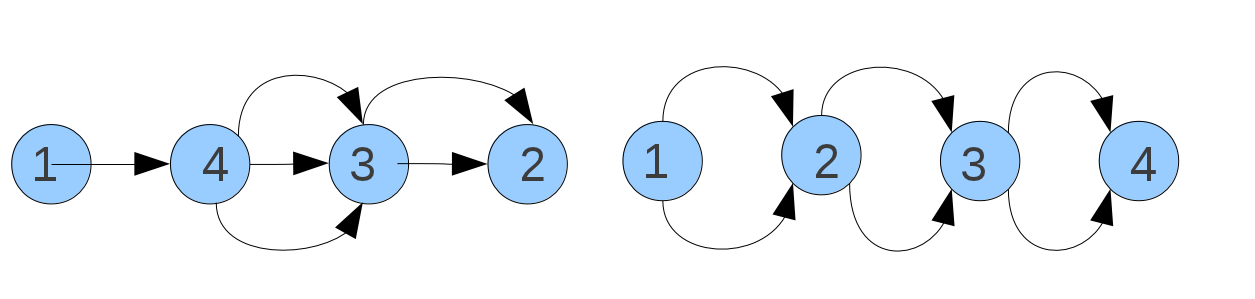
\includegraphics[scale=0.40]{Graphe.png}
\end{center}
\end{figure} 
Dans un cas on peut voir que le nombre de chemins est seulement de 1 pour le premier graphe car l'algorithme ne trouve qu'un chemin à partir de 1 et ne cherche pas les chemins existants vers tous nœuds (bien qu'il y en ait en fait 6).  Tandis que pour le  second parcours l'on obtient 8 chemins à parcourir.
Je ne me sens pas personnellement capable de donner la plus grande quantité de chemins pour un graphe étant donné le nombre de nœuds et le nombre d'arc, je vais donc cherché un  cas qui entraîne un fort nombre de chemins. Un cas simple à étudier est un cas similaire au second exemple;c'est-à-dire un graphe ou chaque nœuds a tous ses arcs qui pointe vers le nœud « suivant ». Donc si $N<2A$ on peut faire que chaque nœud a en moyenne $\frac{A}{N-1}$ arcs sortants soit $(\frac{A}{N-1})^{N-1}$ chemins, ou si $N>2A$ $2^{\frac{A}{2}}$ chemins en répartissant correctement les arcs. Il faut de plus ajouter à cela la mise à jour du meilleur chemin stocké dans une liste qui dans le pire des cas est faite à chaque fois.
Le nombre de chemins est donc un paramètre exponentiel mais qui pourra énormément varié selon la forme du graphe, la ville de départ et la ville d'arrivée. Ce facteur exponentiel risque d'être cependant souvent présent dans des graphes fortement connexes.
\section{Conclusion}%% methode la plus efficace
methode la plus efficacemethode la plus efficacemethode la plus efficacemethode la plus efficacemethode la plus efficacemethode la plus efficacemethode la plus efficace


\clearpage


